\documentclass[12pt,a4paper,twoside]{report}
\usepackage[margin=1in]{geometry}

\usepackage{fancyhdr, lastpage}
\pagestyle{fancy}
\fancyfoot{}

\usepackage{xargs}
\usepackage[pdftex,dvipsnames]{xcolor}
\usepackage{setspace}
\doublespacing

\usepackage[utf8]{inputenc}
\usepackage[T1]{fontenc}
\usepackage{textcomp}
\usepackage{amsmath,amssymb,mathtools}


% figure support
\usepackage{import}
\usepackage{xifthen}
\pdfminorversion=7
\usepackage{pdfpages}
\usepackage{transparent}
%\newcommand{\incfig}[1]{%
%	\def\svgwidth{\columnwidth}
%	\import{./figures/}{#1.pdf_tex}
%}

\newcommand{\incfig}[2][1]{%
    \def\svgwidth{#1\columnwidth}
    \import{./figures/}{#2.pdf_tex}
}
\usepackage{float}

%Options: Sonny, Lenny, Glenn, Conny, Rejne, Bjarne, Bjornstrup
%\usepackage[Glenn]{fncychap}

%%%%%%%%%%%%%%%%%%%%%%%%%%%%%%
%%%%%%%%%%%%%%%%%%%%%%%%%%%%%%
\usepackage[framemethod=TikZ]{mdframed}

%%%%%%%%%%%%%%%%%%%%%%%%%%%%%%
%Theorem
\newcounter{theo}[section] \setcounter{theo}{0}
\renewcommand{\thetheo}{\arabic{section}.\arabic{theo}}
\newenvironment{theo}[2][]{%
\refstepcounter{theo}%
\ifstrempty{#1}%
{\mdfsetup{%
frametitle={%
\tikz[baseline=(current bounding box.east),outer sep=0pt]
\node[anchor=east,rectangle,fill=blue!20]
{\strut Theorem~\thetheo};}}
}%
{\mdfsetup{%
frametitle={%
\tikz[baseline=(current bounding box.east),outer sep=0pt]
\node[anchor=east,rectangle,fill=blue!20]
{\strut Theorem~\thetheo:~#1};}}%
}%
\mdfsetup{innertopmargin=10pt,linecolor=blue!20,%
linewidth=2pt,topline=true,%
frametitleaboveskip=\dimexpr-\ht\strutbox\relax
}
\begin{mdframed}[]\relax%
\label{#2}}{\end{mdframed}}

%%%%%%%%%%%%%%%%%%%%%%%%%%%%%%
%Result
\newenvironment{rslt}[1][]{%
\ifstrempty{#1}%
{\mdfsetup{%
frametitle={%
\tikz[baseline=(current bounding box.east),outer sep=0pt]
\node[anchor=east,rectangle,fill=blue!20]
{\strut Result};}}
}%
{\mdfsetup{%
frametitle={%
\tikz[baseline=(current bounding box.east),outer sep=0pt]
\node[anchor=east,rectangle,fill=blue!20]
{\strut Result:~#1};}}%
}%
\mdfsetup{innertopmargin=10pt,linecolor=blue!20,%
linewidth=2pt,topline=true,%
frametitleaboveskip=\dimexpr-\ht\strutbox\relax
}
\begin{mdframed}[]\relax%
}{\end{mdframed}}

%%%%%%%%%%%%%%%%%%%%%%%%%%%%%%
%Lemma
\newcounter{lem}[section] \setcounter{lem}{0}
\renewcommand{\thelem}{\arabic{section}.\arabic{lem}}
\newenvironment{lem}[2][]{%
\refstepcounter{lem}%
\ifstrempty{#1}%
{\mdfsetup{%
frametitle={%
\tikz[baseline=(current bounding box.east),outer sep=0pt]
\node[anchor=east,rectangle,fill=green!20]
{\strut Lemma~\thelem};}}
}%
{\mdfsetup{%
frametitle={%
\tikz[baseline=(current bounding box.east),outer sep=0pt]
\node[anchor=east,rectangle,fill=green!20]
{\strut Lemma~\thelem:~#1};}}%
}%
\mdfsetup{innertopmargin=10pt,linecolor=green!20,%
linewidth=2pt,topline=true,%
frametitleaboveskip=\dimexpr-\ht\strutbox\relax
}
\begin{mdframed}[]\relax%
\label{#2}}{\end{mdframed}}
%%%%%%%%%%%%%%%%%%%%%%%%%%%%%%
%Proof
\newenvironment{prf}[1][]{%
\ifstrempty{#1}%
{\mdfsetup{%
frametitle={%
\tikz[baseline=(current bounding box.east),outer sep=0pt]
\node[anchor=east,rectangle,fill=red!20]
{\strut Proof};}}
}%
{\mdfsetup{%
frametitle={%
\tikz[baseline=(current bounding box.east),outer sep=0pt]
\node[anchor=east,rectangle,fill=red!20]
{\strut Proof:~#1};}}%
}%
\mdfsetup{innertopmargin=10pt,linecolor=red!20,%
linewidth=2pt,topline=true,%
frametitleaboveskip=\dimexpr-\ht\strutbox\relax
}
\begin{mdframed}[]\relax%
}{$\null\hfill \blacksquare$\end{mdframed}}

%\newcounter{prf}[section]\setcounter{prf}{0}
%\renewcommand{\theprf}{\arabic{section}.\arabic{prf}}
%\newenvironment{prf}[2][]{%
%\refstepcounter{prf}%
%\ifstrempty{#1}%
%{\mdfsetup{%
%frametitle={%
%\tikz[baseline=(current bounding box.east),outer sep=0pt]
%\node[anchor=east,rectangle,fill=red!20]
%{\strut Proof~\theprf};}}
%}%
%{\mdfsetup{%
%frametitle={%
%\tikz[baseline=(current bounding box.east),outer sep=0pt]
%\node[anchor=east,rectangle,fill=red!20]
%{\strut Proof~\theprf:~#1};}}%
%}%
%\mdfsetup{innertopmargin=10pt,linecolor=red!20,%
%linewidth=2pt,topline=true,%
%frametitleaboveskip=\dimexpr-\ht\strutbox\relax
%}
%\begin{mdframed}[]\relax%
%\label{#2}}{\qed\end{mdframed}}
%%%%%%%%%%%%%%%%%%%%%%%%%%%%%%
%%%%%%%%%%%%%%%%%%%%%%%%%%%%%%


%%%%%%%%%%%%%%%%%%%%%%%%%%%%%%
%%%%%%%%%%%%%%%%%%%%%%%%%%%%%%
%%%%%%%%%%%%%%%%%%%%%%%%%%%%%%
%SECTION FORMATTING
\usepackage{tikz}
\usepackage[explicit]{titlesec}
\titleformat{\chapter}
{\scshape\bfseries\LARGE}{\thechapter}{1pt}
{\begin{tikzpicture}
    \node[yshift=-3cm] at (current page.north west)
      {\begin{tikzpicture}
        \draw[color=Red!40, fill=Red!40] (0.02,0) rectangle
	    (.7\paperwidth, 0.1);
        \node[yshift=1.9ex, anchor=west, rectangle, color=Red!40, fill=Red!40]
              {\color{black}#1};
       \end{tikzpicture}
      };
   \end{tikzpicture}
} %not sure why my compiler doesn't like this but the parentheses is necessary
\titlespacing*{\chapter}{0pt}{30pt}{-10pt}

\titleformat{\section}
{\Large}{\thesection}{1pt}
{\begin{tikzpicture}
    \node[yshift=-3cm] at (current page.north west)
      {\begin{tikzpicture}
        \draw[color=Blue!20, fill=Blue!20] (0.02,0) rectangle
	    (.7\paperwidth, 0.1);
        \node[yshift=1.9ex, anchor=west, rectangle, color=Blue!20, fill=Blue!20]
              {\color{black}#1};
       \end{tikzpicture}
      };
   \end{tikzpicture}
} %not sure why my comiler doesn't like this but the parentheses is necessary
\titlespacing*{\section}{0pt}{30pt}{-10pt}

\usepackage[none]{hyphenat}

%%%%%%%%%%%%%%%%%%%%%%%%%%%%%%
%\usepackage[colorinlistoftodos,prependcaption,textsize=tiny]{todonotes}
%\newcommandx{\unsure}[2][1=]{\todo[linecolor=red,backgroundcolor=red!25,bordercolor=red,#1]{#2}}
%\newcommandx{\change}[2][1=]{\todo[linecolor=blue,backgroundcolor=blue!25,bordercolor=blue,#1]{#2}}
%\newcommandx{\info}[2][1=]{\todo[linecolor=OliveGreen,backgroundcolor=OliveGreen!25,bordercolor=OliveGreen,#1]{#2}}
%\newcommandx{\improvement}[2][1=]{\todo[linecolor=Plum,backgroundcolor=Plum!25,bordercolor=Plum,#1]{#2}}
%\newcommandx{\thiswillnotshow}[2][1=]{\todo[disable,#1]{#2}}
%%%%%%%%%%%%%%%%%%%%%%%%%%%%%%

\usepackage{hyperref}

\newcommand\N{\ensuremath{\mathbb{N}}}
\newcommand\R{\ensuremath{\mathbb{R}}}
\newcommand\Z{\ensuremath{\mathbb{Z}}}
\renewcommand\O{\ensuremath{\emptyset}}
\newcommand\Q{\ensuremath{\mathbb{Q}}}
\newcommand\C{\ensuremath{\mathbb{C}}}
\renewcommand\P{\ensuremath{\mathcal{P}}}

\pdfsuppresswarningpagegroup=1



\title{Chapter 1}
\author{Logan Rosentreter}
\date{\today} %\today

\rhead{Rosentreter, \thepage\ of \pageref{LastPage}}
\lhead{STAT 480} %class
\chead{Chapter 1} %document

\begin{document}
\maketitle\thispagestyle{fancy}
\chapter*{Probability}
\section*{Intro}
Probability is a measure of one's belief in the occurrence of future events
\subsubsection*{e.g.}
a policy holder making a claim in the next year
\section*{How to assign probabilities?}
\begin{enumerate}
    \item subjectively
    \item relative frequency
	\begin{itemize}
	    \item repeat the study condition (identical) for M times
	    \item record times event occurred (m)
	    \item probability = relative frequency = m / M where $\lim_{M \to \infty} m / M = P(A)$
	\end{itemize}
    \item Axiomatic Model Based
	\begin{itemize}
	    \item use mathematical theory to assign probabilities (what we will learn)
	\end{itemize}
\end{enumerate}
\section*{Notation}

Def : A random experiment is an experiment that produces outcomes that can't be predicted w/ certainty

Def : A performance of such experiment : trial

Def : A result : Outcome

Def : Sample Space : set of all possible outcomes of an experiment
\begin{itemize}
    \item Denote $S$
\end{itemize}
Ex : Toss a coin 3 times.
\begin{equation*}
    S = 
    \begin{Bmatrix} 
	\text{HHH HHT HTH HTT} \\
	\text{THH THT TTH TTT}
    \end{Bmatrix}
\end{equation*}

Ex : number of positive tests during a week. $S = \{0, 1, 2, \ldots \}$  
 
Ex : highest temp. on labor day. $S = \{40 < \omega < 120 \}$ 

Ex : An event is a subset of sample space, $S$, as $(A, B, C \ldots) \subseteq S$

Def :  $\omega$ : "omega" an outcome occurs
 \begin{itemize}
    \item if $A$ contains $\omega$, we say $A$ occurred
    \item if $A$ does not contain $\omega$, $A$ did not occur
\end{itemize}
i.e. $\omega  \in A, A \text{ occurred}$, $\omega \not\in A, A \text{ did not occur}$

e.g. Toss coin 3 times. $A = $ getting @ least 2 heads

$A = \{ HHH, HHT, HTH, THH \}$. If I toss the coin 3 times and get  $HTH$, then $A$ occurred if I get $TTH$, $A$ did not occur

\chapter*{Set Theory}
\begin{itemize}
    \item $A$ is a subset of $S$ if $\omega \in A \implies \omega \in S$ 
    \item Union : $A \cup B = \{ \omega : \omega \in A \text{ or } \omega \in B \}$
    \item intersection : $A \cap B = \{ \omega : \omega \in A \text{ and } \omega \in B \}$
    \item complement : $\overline{A} = \{ \omega \in S : \omega \not\in A \}$
\end{itemize}

Notate : $A_1 \cap A_2 \cap \ldots \cap A_n = \bigcap_{i = 1}^n A_i$

Notate : $A_1 \cup A_2 \cup \ldots \cup A_n = \bigcup_{i = 1}^n A_i$

Notate : $\O = $ null event (empty set)

Notate : $S = $ sure event (always occur)

Def : An event is called elementary (simple) event if it contains only 1 outcome

Def : mutually exclusive (disjoint)

\begin{itemize}
    \item $A \cap B = \O \implies \text{ no common outcome}$
\end{itemize}

$A_1, A_2, \ldots, A_k$ are all mutually exclusive if they are pairwise mutually exclusive i.e. $A_i \cap A_j = \O$ for all $i \not= j$

Ex : Toss a coin 3 times

A : at least 2 heads
\[
    A = \{HHH, HHT, HTH, THH \}
\] 

B : 1st toss = tails
\[
    B = \{ THH, THT, TTH, TTT \}
\] 
\begin{align*}
    A \cap B &= \{ THH \} \implies \text{ not mutually exclusive} \\
    A \cup B &= \{ HHH, HHT, HTH, THH, THT, TTH, TTT \} \\
    \overline{A \cup B} &= \{ HTT \} \\
    \overline{A} &= \{ HTT \} \\
    \overline{B} &= \{ HTT, HHH, HHT, HTH \}
\end{align*}
\subsubsection*{DeMorgan's Law}

\begin{align*}
    \overline{A \cup B} = \overline{A} \cap \overline{B} \\
\overline{A \cap B} = \overline{A} \cup \overline{B}
\end{align*}

\section*{Definition of Probability}

$S$ Sample Space - all outcomes of an experiment

$A$ event, $A \subseteq S$ 

$B = $ set of all possible events

$P  = $ probability set function if 

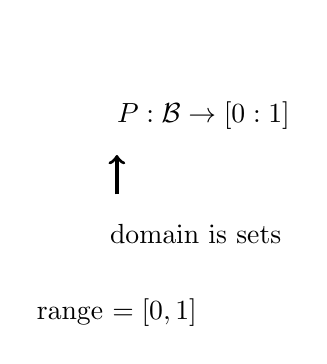
\begin{tikzpicture}
    \node at (0,1) {};
    \node at (1.1,0) {$P : \mathcal{B} \to [0:1]$};
    \draw[very thick, ->] (0,-1) -- (0,-0.5);
    \node at (1,-1.5) {domain is sets};
    \node at (0,-2.5) {range $ = [0,1]$};
\end{tikzpicture}

\subsection*{Kolmogrov's axioms}

\begin{enumerate}
    \item $P(A) \ge 0 \text{ for all } A \in B$ 
    \item $P(S) = 1$
    \item if $A_1, A_2, \ldots \leftarrow \mathcal{B}$ are mutually exclusive, then
	\[
	    P(\bigcup_{i = 1}^\infty A_i) = \sum\limits_{i=1}^{\infty} A_i
	\] 
\end{enumerate}

\subsection*{Remark}

$P(A)$ is the probability of $A$ 

\begin{rslt}
    $P(\O) = 0$
\end{rslt}
\begin{prf}
\begin{align*}
    S \cap \O &= \O \\
    P(S \cap \O) &= P(S) + P(\O) \\
    P(S) &= P(S) + P(\O) \\
    P(\O) &= 0
\end{align*}
\end{prf}
\section*{Discrete Sample Space}

Assign probability to single outcomes (elementary / simple event)

i.e.
 \begin{align*}
     P( \{ e_i \} ) &= P_i \\
     P_i &\ge 0 \text{ for all } i \\
     \sum\limits_{i=1}^{\infty} P_i &= 1 = P(S) \\
     P(A) &= \sum\limits_{e_i \in A} P( \{ e_i \} )
\end{align*}

e.g. Toss a coin 3 times
\begin{align*}
    P( \{ HHH \} ) &= P( \{ HHT \} ) = \ldots = 1/8 \\
    A &: \text{ At least 2 heads} \\
    A &= \{ HHH, HHT, HTH, THH \} \\
    P(A) &= P( \{ HHH \} ) + P( \{ HHT \} ) + \ldots = 1/8 + 1/8 + \ldots + 1/8 = 1/2
\end{align*}

\section*{Equal Probability Model (Classical) <Discrete Space>}
Discrete Sample Space $S$ contain $N$ outcomes $(N < \infty)$ each outcome is equally likely

i.e.
\begin{align*}
    P_1 &= P_2 = \ldots = P_n \\
    P_i &> 0 \\
    \sum P_i &= 1, \text{ then } \\
    P_i = 1/N \text{ for all } i \\
P(A) &= \sum\limits_{i=1}^{n(A)} 1/N = \frac{n(A)}{N} \text{ where } n(A) = \text{ \# of outcomes in } A \\
\end{align*}
\end{document}
